% Section content template for individual Educative lessons
% This file contains the actual content for a specific section
% Generated from Educative API section content

% Section: Requirements for the Restaurant Management System
% Section ID: 5592799430049792
% Section Slug: requirements-for-the-restaurant-management-system
% Generated: 2025-12-14T12:22:50.999869

In this lesson, we'll list the restaurant management system design requirements. This is a crucial step since requirements define the scope of a problem. Therefore, getting them right from the interviewer and understanding them well will make the design of the rest of the system smooth and easy.
\\
We'll use the notational convention to identify each requirement with a unique label, ``Rn,'' where ``R'' is short for requirement and ``n'' is a natural number.

\subsection{Requirement collection}\label{vbritmRUh3Tv6frjGhagR}

% \vspace{-1.0\baselineskip}
\noindent
\begin{minipage}[t]{0.48\textwidth}\vspace{0pt}
\textbf{R1:} The restaurant can have multiple branches.
\\
\textbf{R2:} Each branch will offer a menu with various sections and items.
\\
\textbf{R3:} The server should be able to create an order for a table, add items for each person seated, and update the order as needed.
\end{minipage}
\hfill
\begin{minipage}[t]{0.48\textwidth}\vspace{0pt}
\centering
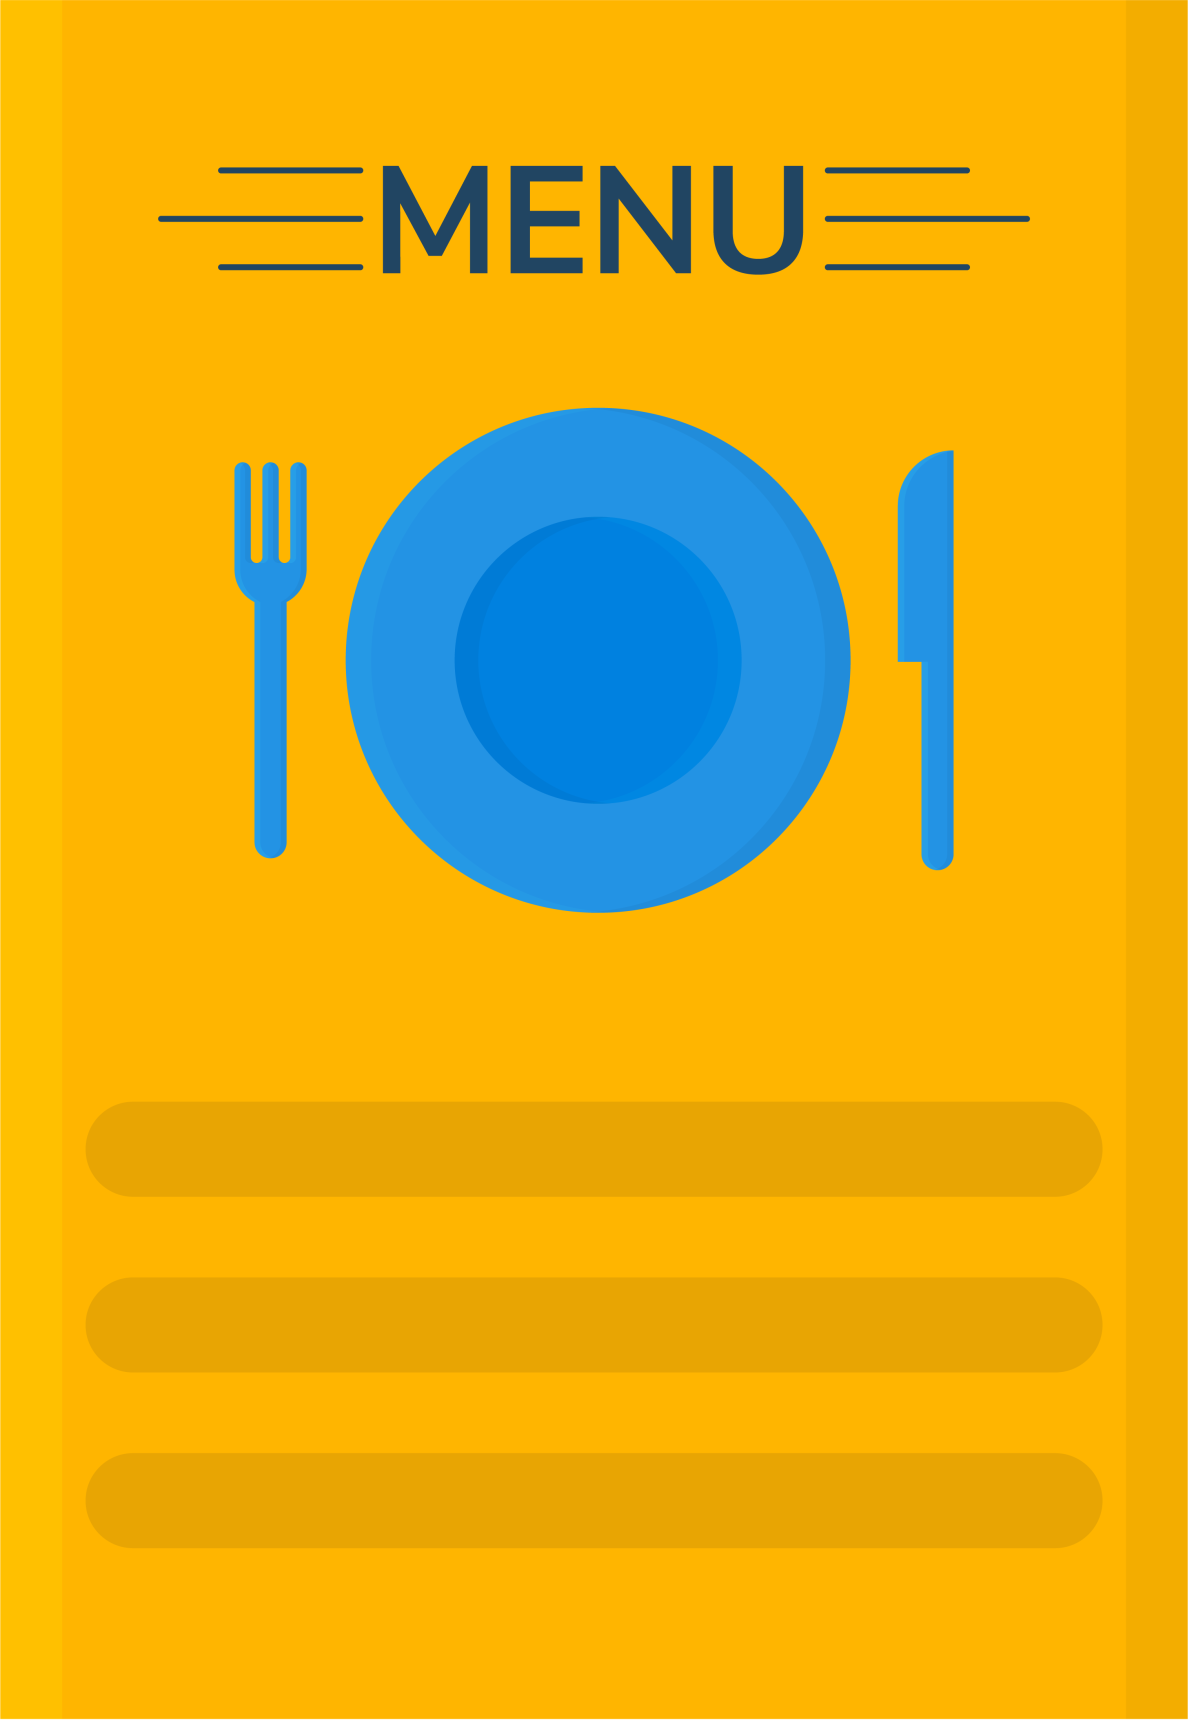
\includegraphics[width=0.5\textwidth]{Images/chapter_21/section_5592799430049792/6261130122231808.png}
\end{minipage}

% \vspace{-1.0\baselineskip}
\noindent
\begin{minipage}[t]{0.48\textwidth}\vspace{0pt}
\textbf{R4:} Each person's order can consist of multiple items, each corresponding to a menu item.
\\
\textbf{R5:} The system should be able to provide information about tables currently available for walk-in customers.
\\
\textbf{R6:} The system should allow for the reservation of tables.
\end{minipage}
\hfill
\begin{minipage}[t]{0.48\textwidth}\vspace{0pt}
\centering
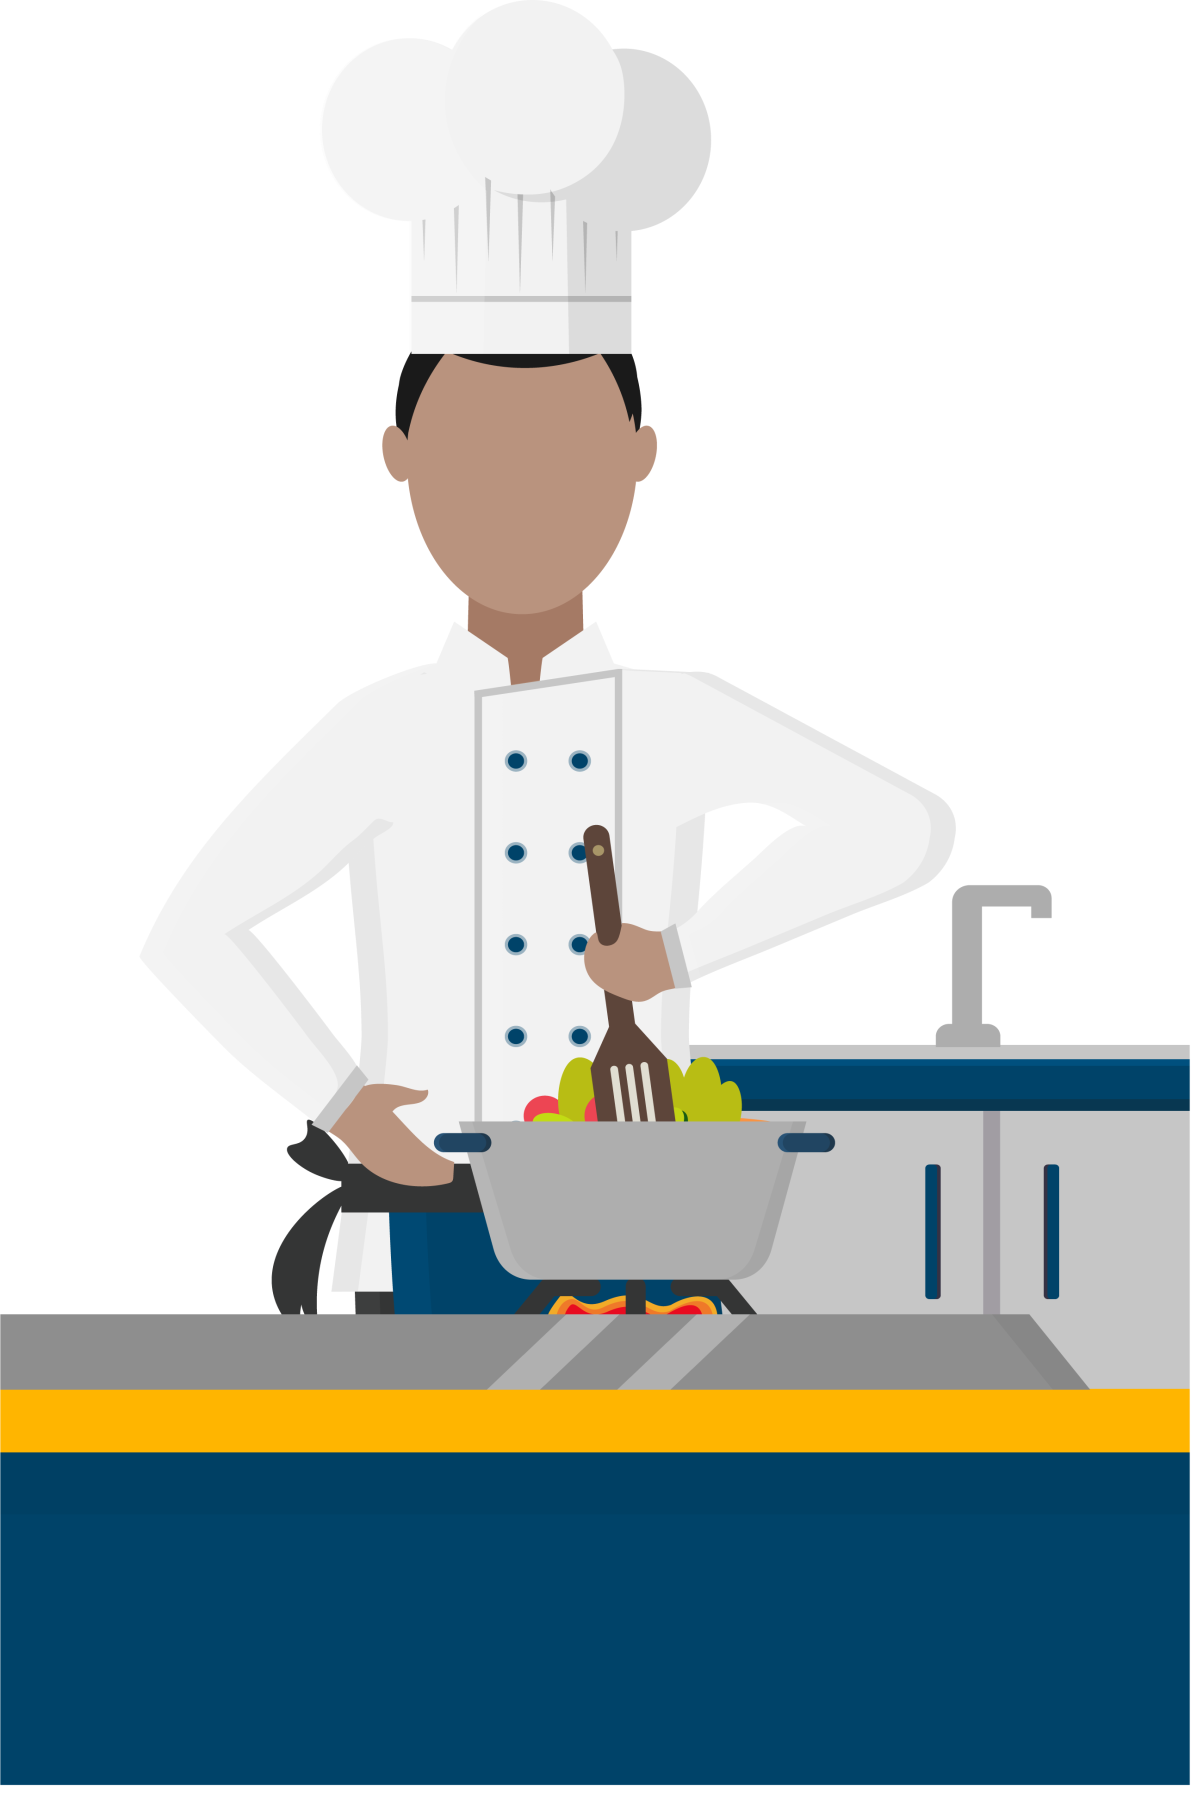
\includegraphics[width=0.5\textwidth]{Images/chapter_21/section_5592799430049792/5837053372923904.png}
\end{minipage}

% \vspace{-1.0\baselineskip}
\noindent
\begin{minipage}[t]{0.48\textwidth}\vspace{0pt}
\textbf{R7:} The receptionist should be able to search for available tables by date and time and make a reservation.
\\
\textbf{R8:} The system should allow customers to make and cancel reservations.
\\
\textbf{R9:} The system should send notifications as the reservation time approaches.
\end{minipage}
\hfill
\begin{minipage}[t]{0.48\textwidth}\vspace{0pt}
\centering
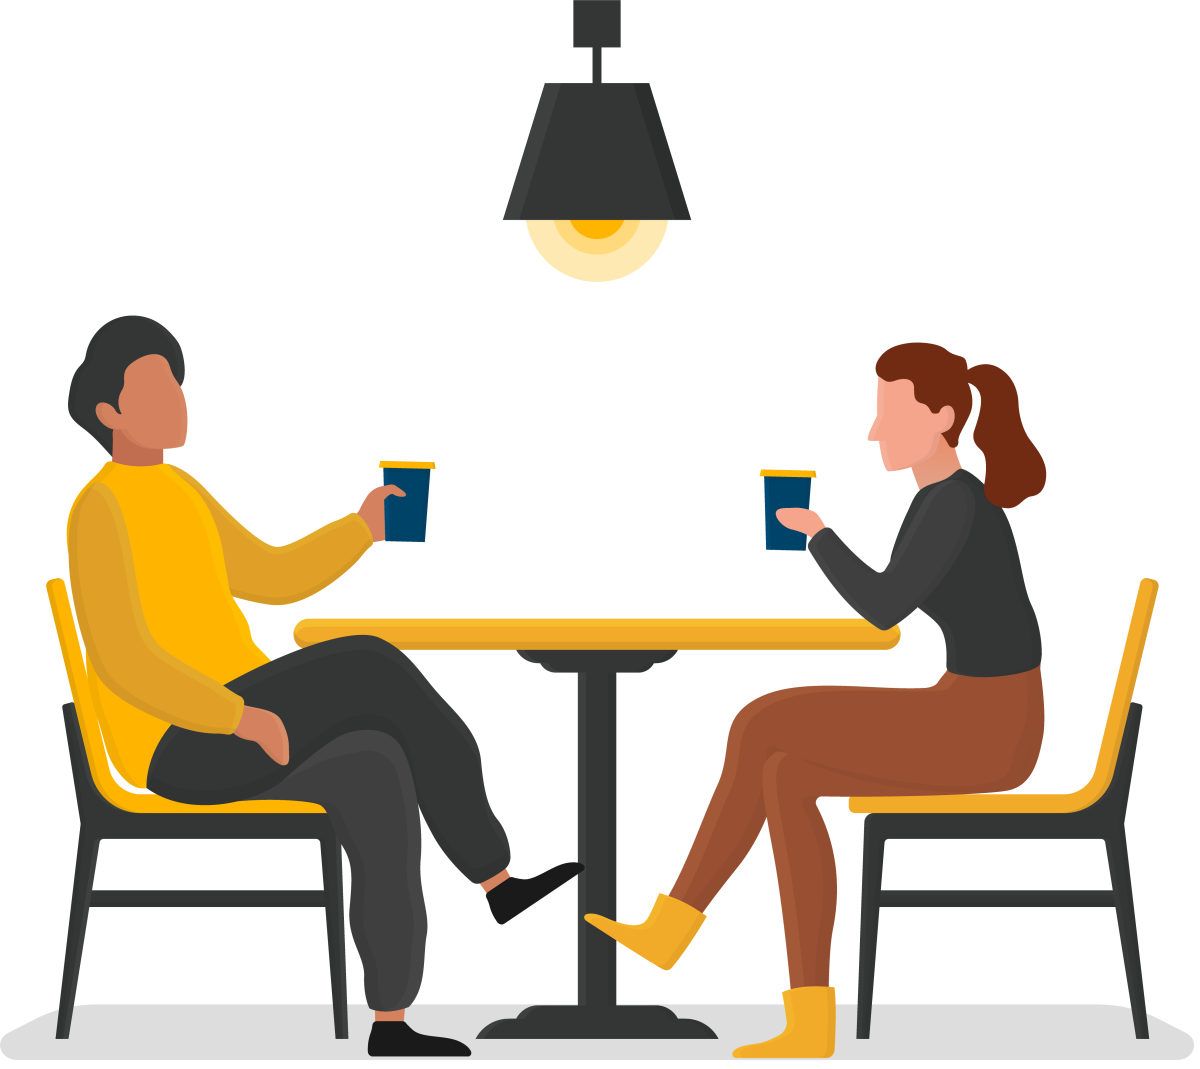
\includegraphics[width=0.5\textwidth]{Images/chapter_21/section_5592799430049792/4639540389347328.png}
\end{minipage}

% \vspace{-1.0\baselineskip}
\noindent
\begin{minipage}[t]{0.48\textwidth}\vspace{0pt}
\textbf{R10:} Customers should be able to pay their bills with credit cards or cash.
\\
\textbf{R11:} Each branch may have a different configuration of tables, managed by the branch manager. The manager can also update the branch's menu.
\\
\textbf{R12:} The system shall allow the server to initiate the payment process for a generated bill by selecting a payment method (credit card or cash), after which the customer completes the payment.
\end{minipage}
\hfill
\begin{minipage}[t]{0.48\textwidth}\vspace{0pt}
\centering
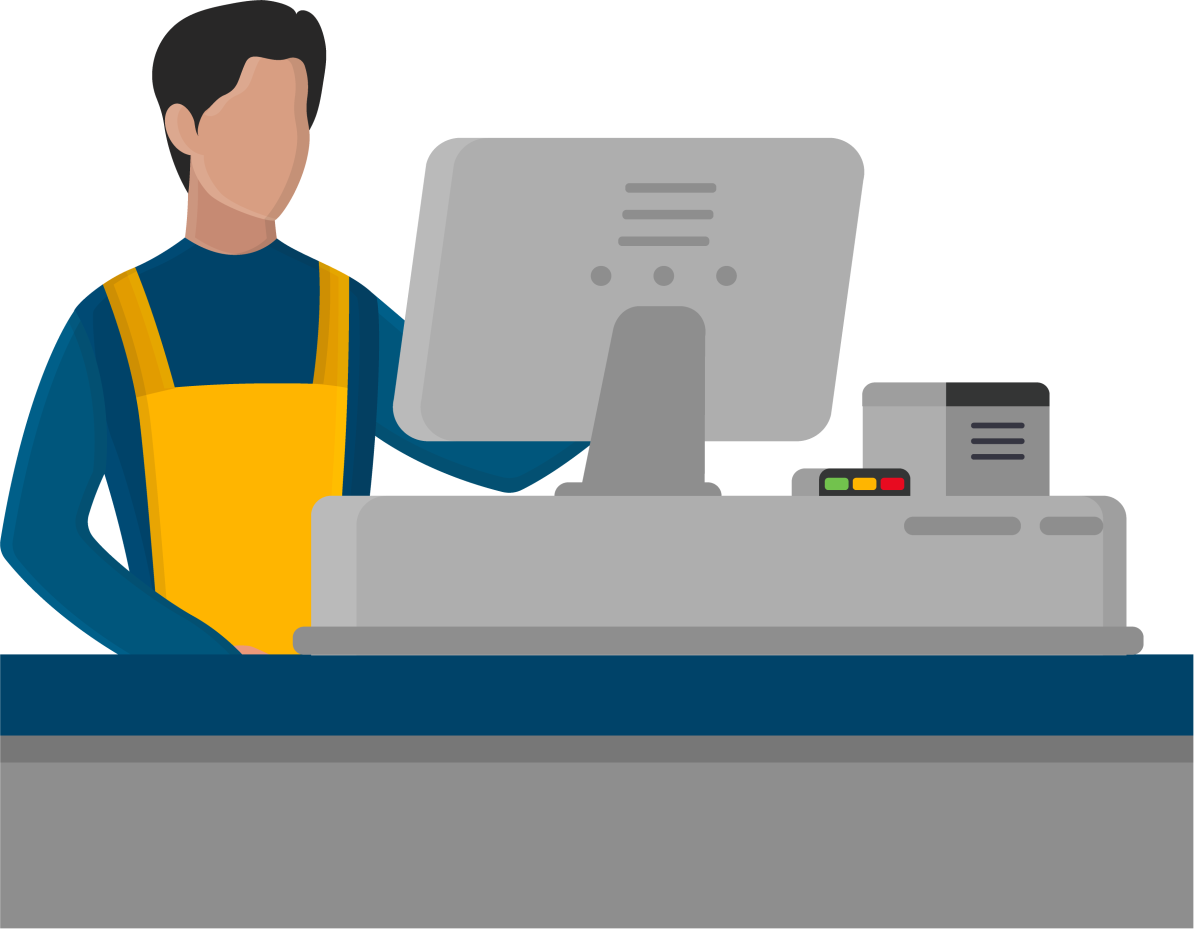
\includegraphics[width=0.5\textwidth]{Images/chapter_21/section_5592799430049792/6355361436270592.png}
\end{minipage}

We've identified our requirements for the problem. In the next lesson, we'll define different use cases of the restaurant management system.

% End of section content